\chapter{Validation Methodology: Simulations Compared with Published Cases}
\label{ch:ch14}

\begin{objectives}
\begin{itemize}[leftmargin=*]
  \item Define verification, calibration and validation for a mechanistic respiratory model.
  \item Describe how simulated patients are compared with published studies.
  \item State the rule that decides whether a model error is an accepted limitation.
\end{itemize}
\end{objectives}

\section{Verification, calibration and validation}
\label{sec:val-terms}
The credibility of a computational model rests on three activities~\citep{asme_vv40,oberkampf2010}. \emph{Verification} asks whether the equations are solved correctly: for VentiVerse, the step-size, solver and CO\textsubscript{2}-conservation checks of \cref{ch:ch03,ch:ch04,ch:ch05}. \emph{Calibration} chooses free parameters so that the model reproduces a named target (\cref{sec:par-calib}). \emph{Validation} compares the model with data that were not used to choose its parameters. ASME V\&V~40 adds that the evidence needed depends on the context of use: what the model is used for, and how much a wrong answer would matter~\citep{asme_vv40}. The intended use here is to explain the physiology of ventilatory failure and to rank the direction of response to therapies, not to predict an individual patient's blood gases for clinical decisions.

\section{Building a validation case}
\label{sec:val-case}
Each disease chapter of Part~V follows the same steps.
\begin{enumerate}[leftmargin=*]
  \item A published study or case report is chosen that reports the patient's characteristics and the blood gases, breathing pattern or effort before and after an intervention.
  \item The patient is built from the reported age, sex, height and weight and the disease parameters of \cref{ch:ch12}, each classed as measured, cited range, fitted or assumption.
  \item The study's protocol is reproduced in a blind simulation: the same ventilator mode and settings, oxygen, posture and, where relevant, a full night of sleep. Outputs are written to CSV files and averaged over the same periods the study measured.
  \item Each published value is paired with its simulated value. Values used for calibration are marked as such; all others are validation pairs.
  \item Overnight oxygen saturation is reported as an oximeter reports it, from an 8-second averaged signal.
\end{enumerate}

\section{Identity charts}
\label{sec:val-identity}
Agreement is shown on identity charts: simulated against published values, with the line of identity and a band of $\pm\SI{10}{\percent}$. \Cref{fig:val-identity} pools every paired PaCO\textsubscript{2} value from the obstructive and neuromuscular disease articles: 26 values from 12 diseases, 16 of them within $\pm\SI{10}{\percent}$. \Cref{tab:val-paco2} summarizes the agreement by disease group.

\begin{figure}[ht]
\centering
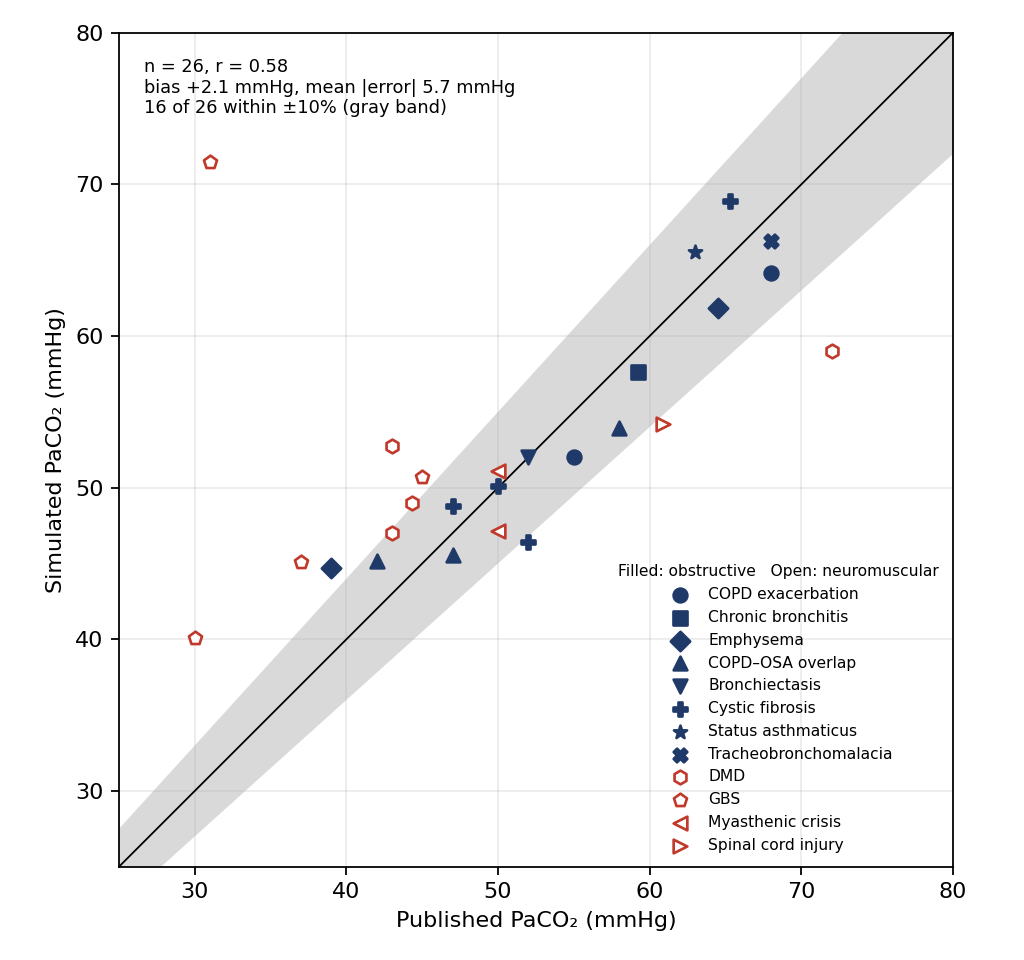
\includegraphics[width=0.72\linewidth]{figures/gen/paco2_identity.png}
\caption{Simulated versus published PaCO\textsubscript{2} for every paired value in the disease validation articles. Filled symbols, obstructive disease; open symbols, neuromuscular disease. Solid line, identity; gray band, $\pm\SI{10}{\percent}$. Simulated values are VentiVerse blind-simulation output; published values are from the studies cited in each disease chapter.}
\label{fig:val-identity}
\end{figure}

\begin{table}[ht]
\centering
\caption{Agreement of simulated with published PaCO\textsubscript{2} (\cref{fig:val-identity}).}
\label{tab:val-paco2}
\small
\begin{tabular}{@{}lcccc@{}}
\toprule
Group & Pairs & Bias (\si{\mmHg}) & Mean absolute error (\si{\mmHg}) & $r$ \\
\midrule
Obstructive (8 diseases) & 15 & $-0.5$ & 2.7 & 0.94 \\
Neuromuscular (4 diseases) & 11 & $+5.6$ & 9.7 & 0.17 \\
All & 26 & $+2.1$ & 5.7 & 0.58 \\
\bottomrule
\end{tabular}
\end{table}

Agreement is close in obstructive disease, where PaCO\textsubscript{2} was the first-ranked calibration target. In neuromuscular disease the model overestimates PaCO\textsubscript{2} in most unsupported patients, and the largest errors come from single case reports.

\section{Direction of the treatment response}
\label{sec:val-direction}
For the intended use, the most important property is that the model changes in the same direction as patients when therapy changes. The disease articles contain 21 published PaCO\textsubscript{2} changes with therapy whose direction can be compared, 19 in obstructive and 2 in neuromuscular disease. In 19 of the 21 the simulated change has the published direction.

\paragraph{Acceptance rule.} An error in magnitude is accepted as a limitation when the simulated response to treatment has the same direction as the published response: the model then ranks therapies correctly even when the size of an effect differs. An error in direction is not accepted. It marks the model as invalid for that use until the cause is found, and it is reported in the disease chapter.

\begin{table}[ht]
\centering
\caption{Responses to therapy with the opposite direction in the model (not accepted).}
\label{tab:val-opposite}
\small
\begin{tabularx}{\linewidth}{@{}X l r r@{}}
\toprule
Study and intervention & Variable & Published & Simulated \\
\midrule
\citet{robinson2000}, oxygen in non-retainers & $\Delta$PaCO\textsubscript{2} (\si{\mmHg}) & $-1.3$ & $+1.7$ \\
\citet{yang2024}, high flow in bronchiectasis & $\Delta$PaCO\textsubscript{2} (\si{\mmHg}) & $-4.0$ & $+0.7$ \\
\citet{appendini1994}, EPAP 4 to \SI{8}{\cmH} in exacerbation & Inspiratory effort & $-37\%$ & $+2\%$ \\
\bottomrule
\end{tabularx}
\end{table}

\section{Sensitivity and identifiability}
\label{sec:val-sens}
The calibration sweeps are one-at-a-time sensitivity analyses across each parameter's published bounds. Neural gain, alveolar dead space, airway resistance and flow-limitation strength have the largest effect on PaCO\textsubscript{2}. Some targets cannot separate parameters: PaCO\textsubscript{2} alone cannot distinguish alveolar dead space from neural drive, because both set alveolar ventilation. Breathing rate, tidal volume and the response to a ventilator change are used together to separate them. Where only one target is available, the parameter is classed as fitted and its comparison is a consistency check.

\begin{summarybox}
Verification shows the equations are solved correctly, calibration chooses free values against named targets, and validation compares the model with data not used for calibration. Pooled PaCO\textsubscript{2} agrees closely in obstructive disease and is overestimated in unsupported neuromuscular disease. Errors in size are accepted when the response to therapy has the published direction; errors in direction are reported as not accepted.
\end{summarybox}
